\subsubsection{Descrizione generale}
Questo servizio svolge l'importante funzione di fornire delle API RESTful al Frontend della piattaforma.
Queste permettono di svolgere le azioni richieste dall'utente, soprattutto l'ottenimento di dati dal database.
Per l'implementazione del servizio è stato scelto il framework FastAPI e l'esecuzione avviene in AWS Fargate.

\subsubsection{Diagramma delle classi}
\begin{figure}[H]
    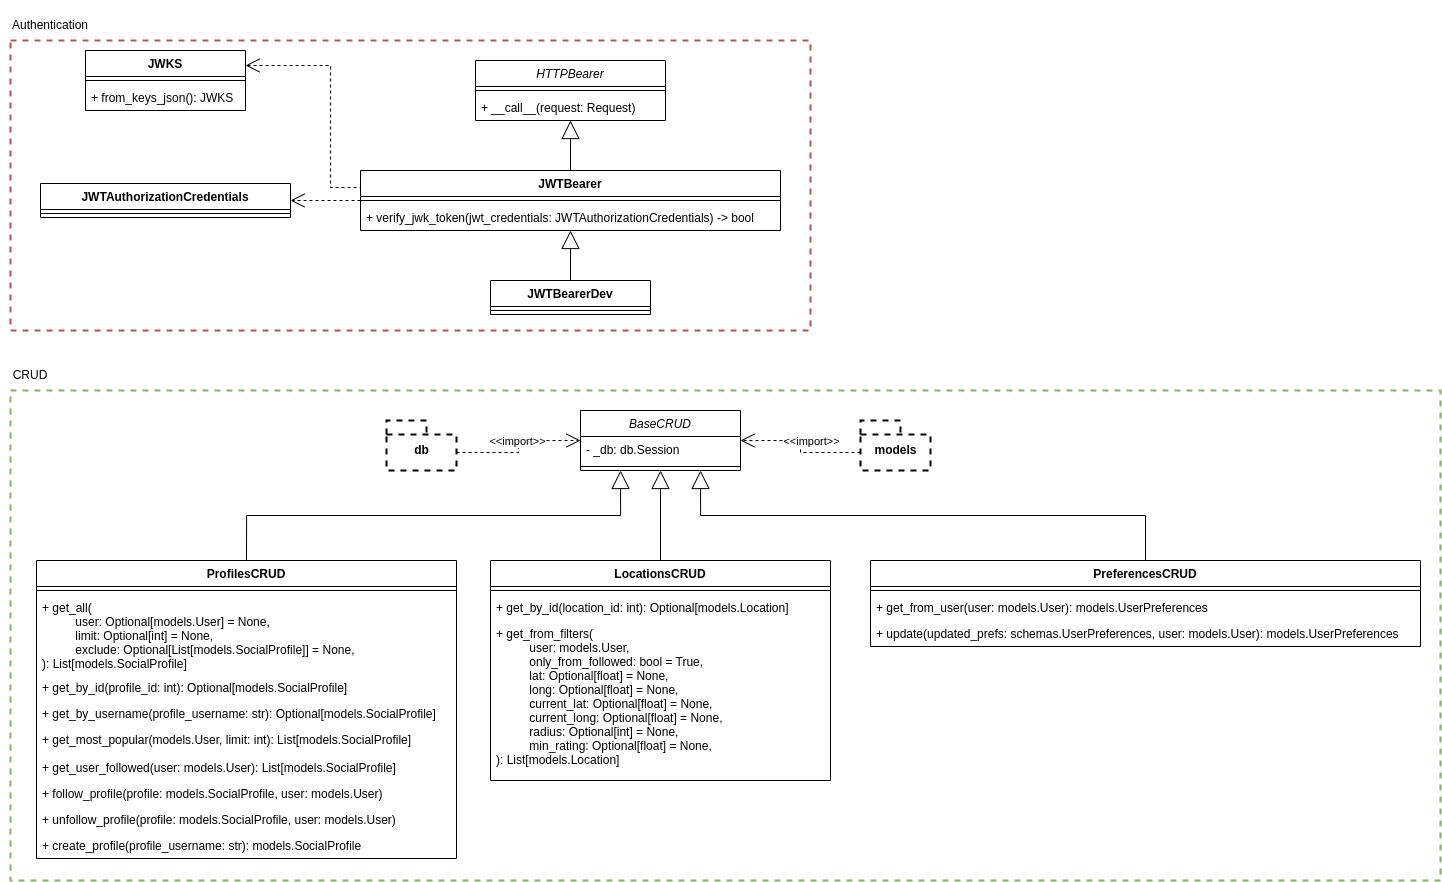
\includegraphics[width=16cm]{sezioni/images/cd_api.png}
    \centering
    \caption{API Service - Diagramma delle classi}
\end{figure}

\subsubsection{Framework FastAPI}
FastAPI è un framework Python moderno, performante e facile da utilizzare per lo sviluppo di API.

\paragraph{Documentazione automatica}\aCapo
Le API vengono documentate automaticamente dal framework, seguendo lo standard OpenAPI.

\subsubsection{AWS Fargate}

\subsubsection{Autenticazione}
